\documentclass[a4paper,11pt]{article}
\usepackage{fullpage}
\usepackage{standalone}
\usepackage[utf8]{inputenc}
\usepackage[british]{babel}
\usepackage{csquotes}
\usepackage[T1]{fontenc}
\usepackage{amsmath}
\usepackage{amssymb}
\usepackage{mathtools}
\usepackage{mathptmx}
\usepackage{natbib}
\usepackage[final,babel]{microtype}
\usepackage[hidelinks]{hyperref}
\usepackage{doi}
\usepackage{siunitx}
\usepackage[margin=1pt]{subcaption}
\usepackage{xcolor}
\PassOptionsToPackage{final}{graphicx}
\usepackage{tikz}
\usetikzlibrary{arrows}
\usetikzlibrary{patterns}
\usepackage{bm}
\usepackage{booktabs}
\usepackage{tabularx}
\usepackage{enumitem}

\title{Monitoring Committee Progress Report \#3\\
\vspace*{1em}
\Large{Numerical Representation of Mountains in Atmospheric Models}}
\author{James Shaw
\vspace{0.5em} \\
\large{Supervisors: Hilary Weller, John Methven, Terry Davies}
\vspace{0.5em} \\
\large{Monitoring Committee: Maarten Ambaum, Paul Williams}}
\date{31st May 2016}

\captionsetup{margin=3pt,font={small}}

\makeatletter
\AtBeginDocument{
  \hypersetup{
    pdftitle = {Monitoring Committee Progress Report \#3},
    pdfauthor = {James Shaw}
  }
}
\makeatother


\newcommand{\TODO}[1]{\textcolor{purple}{TODO: \emph{#1}}}
\begin{document}
\newcommand{\exner}{\Pi}
\maketitle

\section{Introduction}

Next-generation atmospheric models are designed to be more flexible than previous models, so that the choice of mesh and choices of numerical schemes can be deferred or changed during operation \citep{ford2013,theurich2015}.
My PhD project seeks to make numerical weather and climate predictions more accurate by developing new meshes and numerical schemes that are suitable for next-generation models.
In particular, the project addresses the modelling of orographic flows on arbitrary meshes, focusing on three aspects: first, how orography is best represented by a mesh; second, how to accurately advect quantities over orography and, third, how to avoid unphysical solutions in the vertical balance between pressure and temperature.

\subsection*{Representing orography with meshes}

There are two main types of mesh used in atmospheric models: terrain-following meshes and cut cells meshes.
Terrain-following meshes reduce numerical accuracy in the calculation of horizontal pressure gradients \citep{gary1973,zaengl2012} and advection terms \citep{schaer2002}.  Inaccuracies are larger near steep terrain.
The cut cell method is an alternative to terrain-following meshes.  Cut cell meshes are orthogonal everywhere except at the surface so that pressure gradient errors and advection errors are reduced, especially near steep terrain \citep{lock2012,good2014}.  While the cut cell method can reduce numerical errors, cut cell meshes can have arbitrarily small cells which impose severe constraints on the timestep for explicit methods \citep{almgren1997}.

To illustrate the two types of mesh, a wave-shaped mountain with a peak height of \SI{1}{\kilo\meter} is represented using a basic terrain-following mesh (figure~\ref{fig:btf-mesh}) and a cut cell mesh (figure~\ref{fig:cutcell-mesh}).  Notice that the basic terrain-following mesh is severely distorted over steep surfaces while, on the cut cell mesh, small cells are found near the mountain peak.

\subsection*{Advection on arbitrary meshes}
\TODO{what is our scheme?  it's multidimensional (but dimensionally-split schemes can compensate for transverse transport, e.g. bott2010).  it's fairly cheap to compute (but perhaps others are, too, e.g. MPDATA?).  what else is so great about it?}

\TODO{I think I need to justify our scheme by saying that having a multidimensional scheme is important to avoid splitting errors.  then say what other multidimensional schemes exist, what are their pros/cons?  lashley uses a swept-area multidimensional scheme, but it appears to require plenty of recomputation when the wind field changes.}

\TODO{desirable characteristics: conservation, non-oscillatory, accurate (by some norm, often $\ell_2$), efficient computation}

\TODO{what schemes already exist for arbitrary meshes?  what desirable characterstics do they have?  what do they lack?}

\TODO{our scheme is heavily based on lashley2002, who else?  what desirable characteristics does it/should it have?  what does it have that others don't?  what does it lack?}
% see slanted-cell-advection//advection.md notes

\subsection*{Vertical balance on arbitrary meshes}
Some numerical models are susceptible to computational modes which produce unphysical solutions.   Models that have a Lorenz vertical staggering of variables can suffer from one such computational mode \citep{arakawa-konor1996}.  The Charney--Phillips vertical staggering does not suffer from the Lorenz computational mode, but it has only been formulated on structured, quadrilateral meshes.  I intend to develop a generalisation of the Charney--Phillips staggering for arbitrary meshes.

\begin{figure}
	\centering
	\subcaptionbox{Basic terrain-following mesh \label{fig:btf-mesh}}[.32\linewidth]{\includegraphics[width=2in]{../thermalAdvection-mesh-btf-1000m-250dz/constant/mesh.pdf}}
	\subcaptionbox{Cut cell mesh \label{fig:cutcell-mesh}}[.32\linewidth]{\includegraphics[width=2in]{../thermalAdvection-mesh-cutCell-1000m-250dz/constant/mesh.pdf}}
	\subcaptionbox{Slanted cell mesh \label{fig:slantedcell-mesh}}[.32\linewidth]{\includegraphics[width=2in]{../thermalAdvection-mesh-slantedCell-1000m-250dz/constant/mesh.pdf}}
	\caption{Cell edges of basic terrain-following, cut cell and slanted cell meshes having the same wave-shaped mountain profile.  Only the lowest \SI{1.2}{\kilo\meter} in the centre of the domain is shown.  The entire domain is \SI{300}{\kilo\meter} wide and \SI{30}{\kilo\meter} high.  Axis units are \si{\meter}.  Cut cell mesh generated with code kindly provided by TROPOS.}
	\label{fig:meshes}
\end{figure}

\section{Comparison of terrain-following and slanted cell meshes}
The first year of my PhD concentrated on comparing the numerical accuracy on terrain-following and slanted cell meshes.
In the second monitoring committee report (called MC2 hereafter), the slanted cell method was referred to as the cut cell method, but it is necessary to make a distinction between the two methods: cut cell and slanted cell meshes have differences that can be seen by comparing the representation of the same terrain profile using cut cells (figure~\ref{fig:cutcell-mesh}) and slanted cells (figure~\ref{fig:slantedcell-mesh}).

The slanted cell method has advantages over the cut cell method.  First, unlike the construction of cut cell meshes, which can be somewhat involved \citep{hartkopf2011}, I have developed a new technique that makes slanted cell meshes straightforward to construct \citep{shaw-weller2016}.  Second, the slanted cell method does not severely constrain the timestep because thin cells are created that are long in the direction of flow.

Since the previous meeting, the Leibniz Institute for Tropospheric Research (TROPOS) have kindly provided me with their cut cell mesh generator used in the All Scale Atmospheric Model \citep{jaehn2015}.  This generates true cut cell meshes and will enable me to compare test results for cut cell and slanted cell meshes.

Our submission to Monthly Weather Review underwent a third round of revisions after our previous monitoring committee meeting.  These revisions included the development of a new slanted cell mesh generation method which avoided the complex heuristics employed by the previous method (see MC2, section 3).  The article was accepted for publication in February 2016 and is now undergoing prepress proofing.

\section{Improving advection on slanted cell meshes}
My current work focuses on improving the stability and accuracy of a multidimensional advection scheme that is suitable for arbitrary meshes \citep{weller-shahrokhi2014}.  The performance of the advection scheme is being evaluated over steep slopes on terrain-following, cut cell and slanted cell meshes.

The multidimensional advection scheme is an explicit, Eulerian, finite-volume scheme that has a cubic upwind-biased stencil.  Fluxes across faces are approximated using a least squares polynomial fit onto the stencil point values.
On a two-dimensional quadrilateral mesh, the stencil has $4 \times 3$ points in the domain interior (figure~\ref{fig:stencil-interior}), but may include fewer points near the boundaries.  This is a particular concern at the lower boundary where stencils may be smaller and highly distorted (figure~\ref{fig:stencil-lower-boundary}).

\begin{figure}
	\centering
	\subcaptionbox{12-point stencil for face in domain interior \label{fig:stencil-interior}}[.48\linewidth]{\documentclass[tikz]{standalone}
\usepackage{bm}
\begin{document}
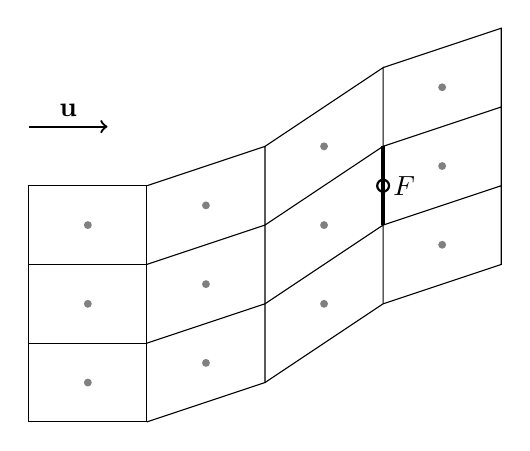
\begin{tikzpicture}[
  scale=0.5,
  cpnt/.style={fill=gray},
]
\draw [thick, ->] (0,7.5) -- (2,7.5) node [midway, anchor=south] {$\mathbf{u}$};

\draw (0,0) -- (3,0) -- (3,2) -- (0,2) -- (0,0);
\draw (0,2) -- (3,2) -- (3,4) -- (0,4) -- (0,2);
\draw (0,4) -- (3,4) -- (3,6) -- (0,6) -- (0,4);

\draw (3,0) -- (6,1) -- (6,3) -- (3,2);
\draw (6,3) -- (6,5) -- (3,4);
\draw (6,5) -- (6,7) -- (3,6);

\draw (6,1) -- (9,3) -- (9,5) -- (6,3);
\draw (9,5) -- (9,7) -- (6,5);
\draw (9,7) -- (9,9) -- (6,7);

\draw (9,3) -- (12,4) -- (12,6) -- (9,5);
\draw (12,6) -- (12,8) -- (9,7);
\draw (12,8) -- (12,10) -- (9,9);

\draw [ultra thick] (9,5) -- (9,7);
\draw [thick] (9,6) circle [radius=0.15] node [anchor=west] {$F$};

\path [cpnt] (1.5,1) circle [radius=0.1];
\path [cpnt] (1.5,3) circle [radius=0.1];
\path [cpnt] (1.5,5) circle [radius=0.1];

\path [cpnt] (4.5,1.5) circle [radius=0.1];
\path [cpnt] (4.5,3.5) circle [radius=0.1];
\path [cpnt] (4.5,5.5) circle [radius=0.1];

\path [cpnt] (7.5,3) circle [radius=0.1];
\path [cpnt] (7.5,5) circle [radius=0.1];
\path [cpnt] (7.5,7) circle [radius=0.1];

\path [cpnt] (10.5,4.5) circle [radius=0.1];
\path [cpnt] (10.5,6.5) circle [radius=0.1];
\path [cpnt] (10.5,8.5) circle [radius=0.1];

\end{tikzpicture}
\end{document}
}
	\subcaptionbox{7-point stencil for face near the lower boundary of a slanted cell mesh.  The ground is shown with diagonal hatching. \label{fig:stencil-lower-boundary}}[.48\linewidth]{\vspace*{2em}\documentclass[tikz]{standalone}
\usepackage{bm}
\usetikzlibrary{patterns}
\begin{document}
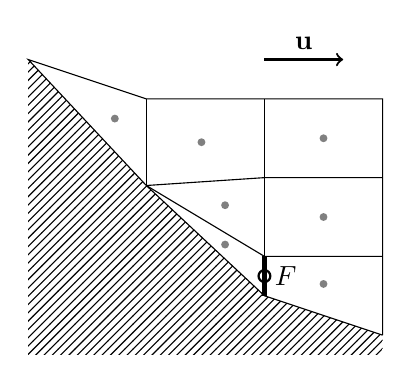
\begin{tikzpicture}[
  scale=0.5,
  cpnt/.style={fill=gray},
]

\draw [thick, ->] (6,7) -- (8,7) node [midway, anchor=south] {$\mathbf{u}$};

\draw (9,0) -- (9,6) -- (3,6) -- (0,7) -- (3,3.8) -- (6,1) -- (9,0);
\draw (3,6) -- (3,3.8);
\draw (6,6) -- (6,1);
\draw (9,2) -- (6,2) -- (3,3.8);
\draw (9,4) -- (6,4) -- (3,3.8);

\fill [pattern=north east lines] (0,7) -- (3,3.8) -- (6,1) -- (9,0) -- (9,-0.5) -- (0,-0.5) -- (0,7);

\draw [ultra thick] (6,1) -- (6,2);
\draw [thick] (6,1.5) circle [radius=0.15] node [anchor=west] {$F$};

\path [cpnt] (2.2,5.5) circle [radius=0.1];

\path [cpnt] (5,2.3) circle [radius=0.1];
\path [cpnt] (5,3.3) circle [radius=0.1];
\path [cpnt] (4.4,4.9) circle [radius=0.1];

\path [cpnt] (7.5,1.3) circle [radius=0.1];
\path [cpnt] (7.5,3) circle [radius=0.1];
\path [cpnt] (7.5,5) circle [radius=0.1];

\end{tikzpicture}
\end{document}
}
	\caption{Two-dimensional stencils used for approximating a value at a face centroid given a set of surrounding cell centre values.  In the two stencils, the face $F$ is shown with a thick line, and the face centroid with an open circle. Cell centres are denoted by grey filled circles.  The direction of the windvector, $\bm{u}$, is shown above both stencils.}
	\label{fig:stencils}
\end{figure}

In the interior of a two-dimensional domain, we fit a polynomial surface to a stencil of a discrete scalar field $\phi$:
\begin{align}
	\phi = a_1 + a_2 x + a_3 y + a_4 x^2 + a_5 x y + a_6 y^2 + a_7 x^3 + a_8 x^2 y + a_9 x y^2
\end{align}
where $a_1 \ldots a_9$ are the unknown coefficients that are calculated from the least squares fit.  It may not be possible to fit all the polynomial terms to a stencil near the lower boundary because it will include fewer points that may be non-uniformly distributed.  With help from Philip Browne, I have developed a mathematical technique that removes certain high-order terms based on the stencil geometry.  We call this technique an `adaptive polynomial fit'.

The adaptive polynomial fit alone is not enough to ensure numerical stability.  I am developing a new procedure that will stabilise the polynomial fit for troublesome stencils.  It is based on constraints derived from a one-dimensional von Neumann analysis of a simplified version of the spatial discretisation.  Compared to the original version of the advection scheme by \citet{weller-shahrokhi2014}, the improved version is stable for a wider range of test cases and has accuracy that is comparable to the original version.  Further work is needed to achieve stability for additional test cases, and give us confidence that the scheme is stable and accurate for arbitrary meshes.

% I could talk about recent work in 1D, potential comparisons with WENO

\section{Future research}
My future work begins with the completion of advection scheme development and the submission of a paper on this topic.  After that, I intend to resume my research into numerical schemes for the Charney--Phillips staggering on arbitrary meshes.

The development of the multidimensional advection scheme, as with so many tasks in life, has proved to be more challenging than initially thought.  The new version of the scheme is already much improved over the original version since it is stable for a larger selection of tests.  However, the scheme is weakly unstable in certain cases (figure~\ref{fig:instability}) and it is not yet clear how to address this issue.  I am collaborating with Tristan Pryer here at Reading, and I am reaching out to other experts in the field for further suggestions.

\begin{figure}
\centering
\subcaptionbox{$t = \SI{1000}{\second}$ (4000 timesteps) \label{fig:instability1000}}[0.32\linewidth]{\hspace*{-1em}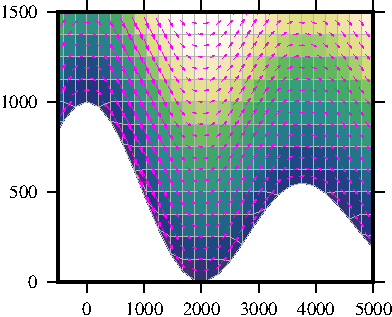
\includegraphics[width=2.25in]{slantedCell1000.pdf}}
\subcaptionbox{$t = \SI{1500}{\second}$ (6000 timesteps) \label{fig:instability1500}}[0.32\linewidth]{\hspace*{1em}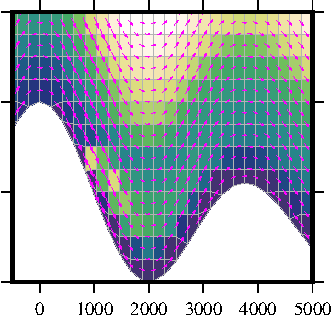
\includegraphics[width=1.9in]{slantedCell1500.pdf}}
\subcaptionbox{$t = \SI{2040}{\second}$ (8160 timesteps) \label{fig:instability2040}}[0.32\linewidth]{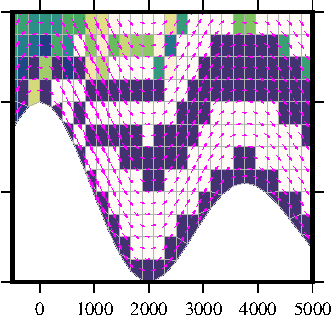
\includegraphics[width=1.9in]{slantedCell2040.pdf}}
%
\vspace{1em} \\
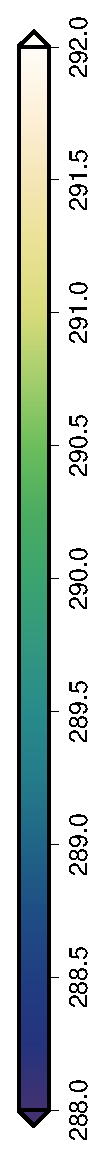
\includegraphics[height=5in,angle=270]{slantedCellLegend.eps}
%
\caption{Development of numerical instability in a test of advection of a stratified thermal field in a prescribed, non-divergent wind field that is tangential to basic terrain-following surfaces.  Errors are too small to be visible at $t = \SI{1000}{\second}$ but, by $t = \SI{1500}{\second}$, erroneously large values have been created near the distorted cells around $x = \SI{1000}{\meter}, z = \SI{600}{\meter}$ that are advected over the lee slopes.  By $t = \SI{2040}{\second}$, the instability is fully-developed, having stripes of error and grid-scale oscillations that propagate in a direction opposite to the wind.  The timestep is \SI{2.5}{\second}.
Cell edges are shown by grey lines.  Wind vectors are drawn at every face using magenta arrows, with the wind speed ranging from \SIrange{10}{13}{\meter\per\second}.  Only the lowest \SI{1.5}{\kilo\meter} of the central domain is shown.  The entire domain is \SI{20}{\kilo\meter} wide and \SI{5}{\kilo\meter} high.  Axis units are \si{\meter}.}
\label{fig:instability}
\end{figure}

MC2 discussed some brief, exploratory work into a generalised Charney--Phillips staggering for arbitrary meshes.  I intend to return to this topic once I am satisfied with the performance of the advection scheme and once I have prepared a paper discussing the advection results.
There are a series of tasks that are required to develop numerical schemes for the generalised Charney--Phillips staggering:
\begin{enumerate}
\item Define the prognostic variables and their arrangement on arbitrary meshes
\item Design a simple numerical scheme for advecting potential temperature
\item Incorporate the advection scheme into the fully-compressible model from \citet{weller-shahrokhi2014}, using a fully-explicit configuration
\item Compare the Lorenz and Charney--Phillips variants of the model by selecting test that excite the Lorenz computational model, such as the standing waves tests from \citet{arakawa-konor1996}
\end{enumerate}
Following this, further tasks should be undertaken if time permits:
\begin{enumerate}[resume]
\item Adapt the multidimensional cubic advection scheme for advecting potential temperature on generalised Charney--Phillips meshes
\item Modify the fully-compressible model to enable a semi-implicit configuration with the Charney--Phillips staggering
\end{enumerate}
\TODO{timescales?}

\section{Training}
This year, I have attended almost all lunchtime and departmental seminars, HHH and mesoscale group meetings.  I take note of analytical techniques that might be useful in future, for example, verifying trends using low pass filters\footnote{The summer NAO in observations and CMIP models: impacts on European precipitation and uncertainties in future projected trends, Ileana Bladé, 7 March 2016}, and solving linear PDEs using Green's functions\footnote{Constraining ocean ventilation pathways and time scales with observations and models, Samar Khatiwala, 21 March 2016}.
Since the second monitoring committee meeting, I have learnt about the Singular Value Decomposition in Numerical Analysis II, which I am using for fitting polynomial surfaces in my own research.
I have also reviewed a manuscript submitted to Monthly Weather Review, and I am keen to get better at critically analysing papers.

Following a talk by Ed Hawkins and Tom Sizmur about online scientific communication, I have been sharing more of my ideas on my blog\footnote{My blog is at \url{datumedge.co.uk}} and on Twitter\footnote{My Twitter username is \href{https://twitter.com/hertzsprrrung}{@hertzsprrrung}}.  I have found Twitter to be especially useful for discovering contacts from a range of disciplines whose interests overlap with my research.

\subsection*{Collaborations}
I have spent some time working with other contacts, sharing ideas about my own and their own research projects:
\begin{itemize}
\item Ram Nair has helped me to arrange a visit to NCAR in June 2016 to present my research and spend time with NCAR staff
\item I am arranging for Simon Clark to visit the department in July 2016.  Simon is a PhD student at Exeter and a YouTube vlogger.  I am organising for him to present a departmental seminar, and to film a radiosonde launch and laboratory demonstrations.
\item I have provided test cases and manuscript reviews for an article about dimensionally-split and multidimensional advection schemes.  I am a coauthor for this article, written with Hilary, her former student Yumeng Chen, and Stephen Pring at the UK Met Office.
\item I intend to collaborate with Hilary's next student, Christiana Skea, who will be investigating variable timestepping for ODEs
\end{itemize}

\footnotesize{
\subsection*{Mathematics modules}
\begin{tabular}{l l l l}
Spring 2016	& MA3NAT & Numerical Analysis II & unassessed \\
Spring 2015	& MAMNSP & Numerical Solution of Partial Differential Equations  & 78\% \\
\end{tabular}

\subsection*{RRDP modules}
\begin{tabular}{l l}
24 Mar 2016	& Voice coaching: looking after your voice \\
26--27 Jan 2016 & Preparing to teach (introduction, marking \& feedback, leading small groups) \\
2 Dec 2015	& An essential guide to critical academic writing \\
17 Nov 2015	& Understanding the UK higher education context \\
19 May 2015	& How to avoid plagiarism \\
10 Mar 2015	& How to write a literature review \\
19 Feb 2015	& How to write a paper \\
\end{tabular}

\subsection*{External courses}
\begin{tabular}{l l}
June 2016 & Dynamical core intercomparison project summer school, NCAR \\
13 May 2016 & Peer review: the nuts and bolts, Sense about Science \\
June 2015 & Advanced numerical methods for Earth-system modelling, ECMWF \\
\end{tabular}

\subsection*{Conferences and workshops}
\begin{tabularx}{\linewidth}{l l X}
October 2016 & Speaker & Numerical and computational methods for simulation of all-scale geophysical flows, ECMWF \\
July 2016 & Attendee & 1st GungHo Network meeting, Daresbury Laboratory \\
November 2015 & Attendee & GungHo workshop on next generation weather and climate prediction, UK Met Office \\
June 2015 & Attendee & Hoskins@70 \\
June 2015 & Poster & SCENARIO DTP conference \\
March 2015 & Speaker & Galerkin methods with applications in weather and climate forecasting, ICMS \\
\end{tabularx}

\subsection*{Presentations}
\begin{tabularx}{\linewidth}{l l X}
23 Mar 2016 & Quo Vadis & Numerical representation of orography in dynamical cores (honourable mention) \\
17 Feb 2016 & PhD group & Multidimensional advection schemes for arbitrary meshes \\
9 Feb 2016 & Mesoscale group & Curl-free pressure gradients for accurate modelling of cold air pools \\
19 Oct 2015 & HHH group & Improving modelled mountain flows with alternative representations of terrain \\
27 Apr 2015 & HHH group & A like-for-like comparison between terrain following and cut cell grids \\
21 Apr 2015 & PhD group & Discrete vector calculus on Arakawa C grids \\
12 Feb 2015 & UK Met office & Poster presentation \\
18 Jan 2015 & PhD group & Python and linux tips \\
17 Dec 2014 & MPECDT jamboree & Poster presentation \\
12 Sep 2014 & Lunchtime seminar  & Gain control of your documents and code: hands-on with revision control and build automation \\
\end{tabularx}

\subsection*{Teaching}
\begin{tabular}{l l l}
Oct 2015 & Teaching assistant & MTMG02 atmospheric physics \\
Sep 2015 & Teaching assistant & NCAS summer school \\
Sep 2014 & Course teacher & MPE python and linux short course \\
\end{tabular}

\subsection*{Outreach}
\begin{tabular}{l l l}
14 Jul 2015 & Schools physicist of the year awards \\
14 Jun 2015 & East Reading festival \\
15 Feb 2015 & Brighton science festival \\
\end{tabular}
}

\bibliographystyle{ametsoc2014}                                                 
\small{\bibliography{references}}

\end{document}
